\chapter{Feedback optimization}


% Single system:

% \begin{enumerate}
%     \item Optimization algorithm: generate a ``reference'' for the control system (algorithmic level).
%     \item Control system: move the robot and use the output as an input of the optimization algorithm (physical level).
% \end{enumerate}

\begin{description}
    \item[Feedback optimization] \marginnote{Feedback optimization}
        Consider a continuous-time non-linear dynamical system:
        \[
            \dot{\x}(t) = f(\x(t), \u(t)) \quad \x(0) = \x_0
        \]
        
        Assume that there exists a steady-state map $h: \mathbb{R}^m \rightarrow \mathbb{R}^n$ (i.e., sort of oracle) that given the input $\bar{\u}$ returns the equilibrium state $\bar{\x}$ associated to it:
        \[
            % \begin{gathered}
                % \forall \bar{\u} \in \mathbb{R}^m: \bar{\u} \mapsto \bar{\x} = h(\bar{\u}) \\
                f(h(\bar{\u}), \bar{\u}) = 0
            % \end{gathered}
        \]
        % Assume that the system is pre-stabilized around the equilibra. i.e., 
        % \[
        %     \begin{split}
        %         \bar{\u} \in \R^m \\
        %         \bar{\u} \mapsto \bar{\x} = h(\bar{\u}) \\
        %         f(\bar{\x}, \bar{\u}) = 0 \\
        %     \end{split}
        % \]
        Moreover, it is assumed that, for any $\bar{\u} \in \mathbb{R}^m$, $\bar{\x} = h(\bar{\u})$ is a globally exponentially stable equilibrium for the system $f(\x(t), \bar{\u})$.

        The goal of feedback optimization is to design a dynamic feedback law $\u(t) = \kappa(\x(t), t)$ such that $\u(t)$ and $\x(t)$ converge to the solution of the problem:
        \[
            \begin{gathered}
                \min_{\z \in \R^n, \u \in \R^m} l(\z) \\
                \text{subject to } \z = h(\u)
            \end{gathered}
        \]
        where $h$ is not explicitly available and the control law can only access the current state $\x(t)$ ($\nabla h$ can however be used).

    \item[Reduced feedback optimization problem] \marginnote{Reduced feedback optimization problem}
        By injecting the constraint of the feedback optimization problem into the cost function, the problem becomes unconstrained:
        \[
            \min_{\u \in \R^m} l(h(\u))
        \]

        % Can apply the gradient method:
        % \[
        %     \u^{k+1} = \u^k - \alpha \nabla h(\u^k) \nabla l(h(\u^k))
        % \]
        and can be solved using the gradient flow:
        \[
            \dot{\u}(t) = -\delta \nabla h(\u(t)) \nabla l(h(\u(t)))
        \]
        where $\delta$ is a hyperparameter (note that it is not the step size as it is not needed in continuous time).

        \begin{figure}[H]
            \centering
            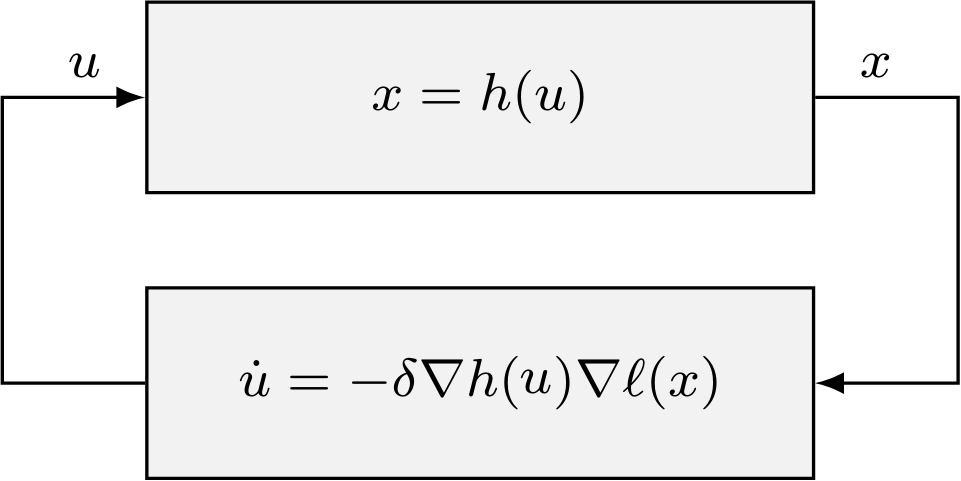
\includegraphics[width=0.35\linewidth]{./img/feedback_reduced_naive.png}
        \end{figure}

        \begin{remark}
            By assumption, $h$ is not available.
        \end{remark}
\end{description}



\section{Centralized feedback optimization}

\begin{description}
    \item[Feedback optimization based on time-scale separation] \marginnote{Feedback optimization based on time-scale separation}
        Gradient flow of the reduced feedback optimization problem where the steady-state $h(\u(t))$ is approximated with the current state $\x(t)$.

        \begin{figure}[H]
            \centering
            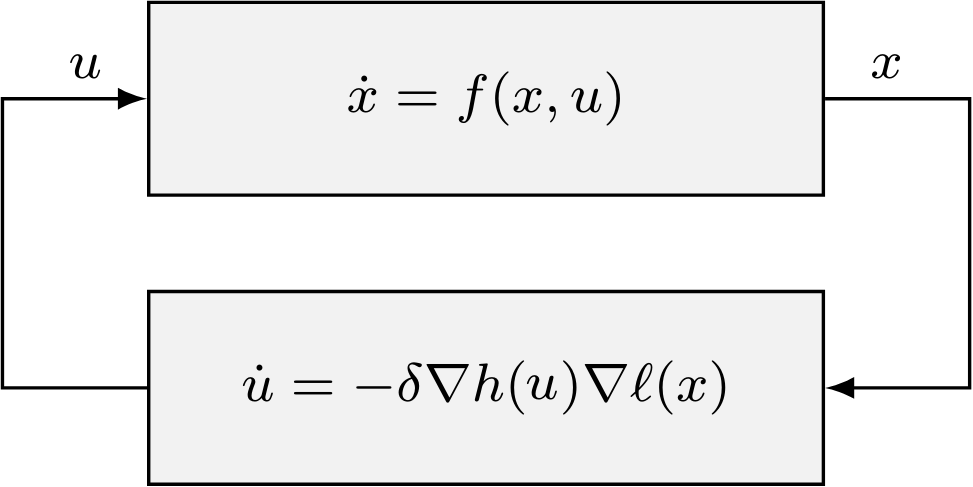
\includegraphics[width=0.35\linewidth]{./img/feedback_timescale.png}
        \end{figure}

        Intuitively, with $\delta > 0$ sufficiently small, we are creating a time-scale separation (i.e., dynamics working on different time-scales) between plant and optimization dynamics:
        \begin{itemize}
            \item The plant $\x(t)$ is a fast dynamics that tracks $h(\u(t))$ (i.e., the equilibrium for the current $\u$) so that $\nabla l(\x(t)) \approx \nabla l(h(\u(t)))$ for the optimization dynamics.
            \item The optimization dynamics is a slow dynamics that changes the input, thus refining the equilibrium that minimizes the loss.
        \end{itemize}
        % (i.e., $\x(t)$ is a fast dynamic tracking  (an equilibrium) and the optimization dynamics is slow that changes the input and thus the equilibrium).

        % If $\delta = 0$, $\dot{\u} = 0$ and $\bar{\x} = h(\bar{\u})$ is globally exponentially stable so that:
        % \[
        %     \x(t) \rightarrow \bar{\x} = h(\bar{\u})
        % \]

    \begin{remark}[Time-scale separation theory]
        Method to analyze a dynamical system by identifying a slow and fast dynamics, and studying them separately. Auxiliary systems are introduced:
        \begin{descriptionlist}
            \item[Boundary-layer system] with $\u$ constant to model the fast system. It is exponentially stable by assumption and can be associated with the Lyapunov function $U(\x)$.
            \item[Reduced system] with the gradient flow without the state $\x$ to model the slow system. It can be shown that it is asymptotically stable with the Lyapunov function $W(\u)$.
        \end{descriptionlist}
        The stability of the whole dynamics is studied by using $U+W$ as Lyapunov function and a sufficiently small $\delta$.

        \begin{figure}[H]
            \centering
            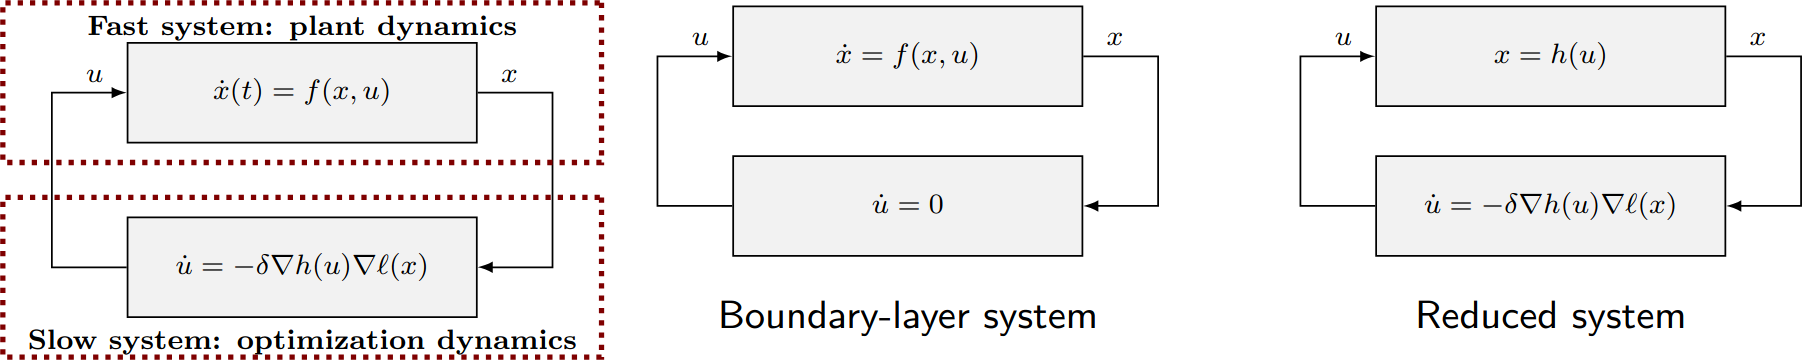
\includegraphics[width=0.95\linewidth]{./img/feedback_time_scale_theory.png}
        \end{figure}
        % \begin{itemize}
        %     \item Slow dynamics: optimization dynamics,
        %     \item Fast dynamics: plant dynamics
        % \end{itemize}
    
        % Treat them separately with two systems:
        % \begin{itemize}
        %     \item Boundary-layer system. It has $\u$ constant (thus exponentially stable by assumption).
        %     \item Reduced system. It is the gradient flow without state $\x$. Can be shown to be asymptotically stable.
        % \end{itemize}
    
        % Use Lyapunov functions $U(\x)$ and $W(\u)$, one for each system, to prove stability. Then, combine then $U+W$ with sufficiently small $\delta$ to show overall stability.
    \end{remark}
\end{description}

\begin{theorem}[Feedback optimization based on time-scale separation convergence]
    Consider a closed-loop system and assume that:
    \begin{itemize}
        \item $\bar{\x} = h(\bar{\u})$ is a globally exponentially stable equilibrium,
        \item $l(h(\cdot))$ is radially unbounded and possibly non-convex,
        \item $\nabla l(h(\cdot))$, $\nabla l$, $h$, and $f$ are Lipschitz continuous.
    \end{itemize}
    It holds that, for a sufficiently small $\delta > 0$, the trajectory $(\x(t), \u(t))$ of the system satisfies:
    \[
        \lim_{t \rightarrow \infty} \texttt{dist}\left( \begin{bmatrix} \x(t) - h(\u(t)) \\ \u(t) \end{bmatrix}, \begin{bmatrix} 0 \\ \u^* \in \mathcal{U}^* \end{bmatrix} \right) = 0
    \]
    where $\texttt{dist}$ is the set distance and $\mathcal{U}^*$ is the set of stationary points of $l(h(\cdot))$.
\end{theorem}



\section{Distributed feedback optimization}

\begin{description}
    \item[Distributed feedback optimization] \marginnote{Distributed feedback optimization} 
        Network of $N$ agents each with dynamics:
        \[
            \dot{\x}_i(t) = f_i(\x_i(t), \u_i(t))
        \]

        The goal is to design a control law $\u_i(t) = \kappa_i(\{ \x_j(t) \}_{j \in \mathcal{N}_i}, t)$ such that $\u_1(t), \dots, \u_N(t)$ and $\x_1(t), \dots, \x_N(t)$ converge to the solution of the problem:
        \[
            \begin{gathered}
                \min_{\substack{(\z_1, \dots, \z_N)\\(\u_1, \dots, \u_N)}} \sum_{i=1}^{N} l_i(\z_i, \sigma(\z)) \\
                \text{subject to } \z_i = h_i(\u_i)
            \end{gathered}
        \]
        where $\sigma(\z) = \frac{1}{N} \sum_{i=1}^{N} \phi_i(\z_i)$ is an aggregation function.

    \item[Reduced distributed feedback optimization] \marginnote{Reduced distributed feedback optimization}
        By injecting the constraint into the cost function, the problem becomes:
        \[
            \min_{(\u_1, \dots, \u_N)} \sum_{i=1}^{N} l_i(h_i(\u_i), \sigma(h(\u)))
        \]
        and can be solved using the parallel gradient flow:
        \[
            \small
            \dot{\u}_i = - \delta_1 \nabla h_i(\u_i) \left( \nabla_{[h_i(\u_i)]} l_i(h_i(\u_i), \sigma(h(\u))) + \left( \sum_{j=1}^{N} \nabla_{[\sigma(h(\u))]} l_j(h_j(\u_j), \sigma(h(\u))) \right) \frac{1}{N}\nabla \phi_i(h_i(\u_i)) \right)
        \]
        where $\delta_1 > 0$ is a hyperparameter.

        \begin{remark}
            This formulation uses $h$ which is not available and requires global information.
        \end{remark}

    \item[Aggregative tracking feedback] \marginnote{Aggregative tracking feedback}
        Use $\x_i$ to approximate $h_i(\u_i)$ and dynamic average consensus for the aggregation function. The dynamics is:
        \[
            \begin{split}
                \dot{\u}_i &= -\delta_1 \nabla h_i(\u_i) \left( \nabla_{[\x_i]} l_i(\x_i, \phi_i(\x_i)+\w_i) + \left( \nabla_{[\phi_i(\x_i)+\w_i]} l_i(\x_i, \phi_i(\x_i)+\w_i) + \v_i \right) \nabla \phi_i(\x_i) \right) \\
                \delta_2 \dot{\w}_i &= - \sum_{j \in \mathcal{N}_i} a_{ij} (\w_i - \w_j) - \sum_{j \in \mathcal{N}_i} a_{ij} (\phi_i(\x_i) - \phi_i(\x_j)) \\
                \delta_2 \dot{\v}_i &= - \sum_{j \in \mathcal{N}_i} a_{ij} (\v_i - \v_j) - \sum_{j \in \mathcal{N}_i} a_{ij} (\nabla_{[\phi_i(\x_i)+\w_i]} l_i(\x_i, \phi_i(\x_i)+\w_i) - \nabla_{[\phi_j(\x_j)+\w_j]} l_j(\x_j, \phi_j(\x_j)+\w_j)) \\
            \end{split}
        \]
        where $\delta_1 > 0$ is used to slow down $\dot{\u}_i$ and $\delta_2 > 0$ to speed up $\dot{\w}_i$ and $\dot{\v}_i$.

        \begin{remark}
            The formulation for dynamic average consensus is for the continuous case with the Laplacian.
        \end{remark}

        \begin{remark}
            The overall system works on three time-scales.
            \begin{figure}[H]
                \centering
                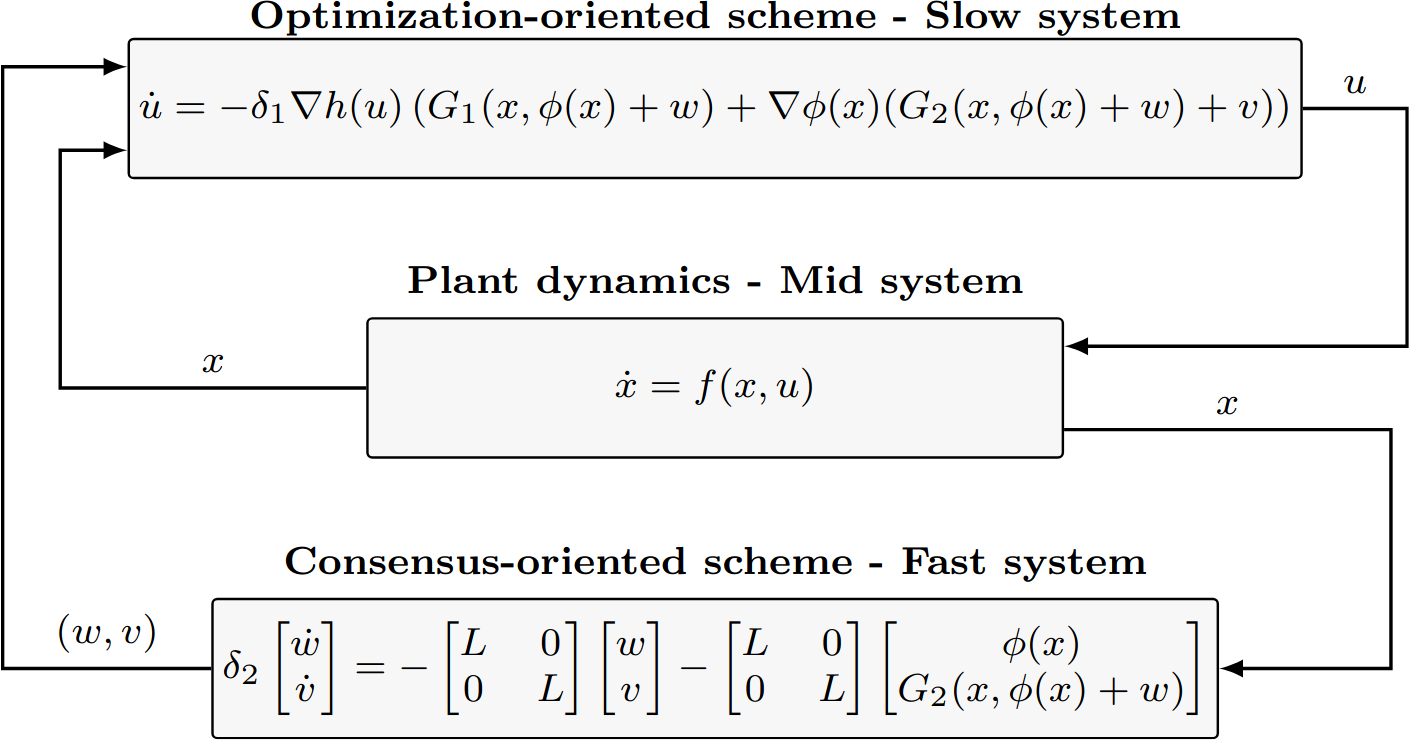
\includegraphics[width=0.6\linewidth]{./img/feedback_distributed.png}
            \end{figure}
        \end{remark}
\end{description}

\begin{theorem}[Aggregative tracking feedback convergence]
    If:
    \begin{itemize}
        \item The aggregative tracking feedback algorithm is initialized so that $\sum_{i=1}^{N} \texttt{col}(\w_i(0), \v_i(0)) = 0$,
        \item $G$ is strongly connected and weight balanced,
        \item $\bar{\x}_i = h_i(\bar{\u}_i)$ is globally exponentially stable,
        \item $\sum_{i=1}^{N} l_i(h_i(\cdot), \sigma(h(\cdot)))$ is radially unbounded and possibly non-convex,
        \item $\nabla_{[\cdot]} l_i$, $\phi_i$, and $h_i$ are Lipschitz continuous.
    \end{itemize}
    Then, for small $\delta_1 > 0$ and $\delta_2 > 0$, the trajectory of the system satisfies:
    \[
        \lim_{t \rightarrow \infty} \texttt{dist}\left( \begin{bmatrix} \x(t) - h(\u(t)) \\ \u(t) \end{bmatrix}, \begin{bmatrix} 0 \\ \u^* \in \mathcal{U}^* \end{bmatrix} \right) = 0
    \]
    where $\mathcal{U}^*$ is the set of stationary points of $\sum_{i=1}^{N} l_i(h_i(\cdot), \sigma(h(\cdot)))$.
\end{theorem}
